\documentclass[ja=minimal]{bxjsarticle}
\usepackage{tikz}
\usepackage{luatexja}
\usepackage{luatexja-fontspec}


\usepackage{pgfplots}
\usepackage{amsmath}
\pgfplotsset{compat=1.18}
\usepackage{graphicx}
\usepackage{multicol}
\usetikzlibrary{intersections,calc,arrows.meta,angles,quotes,patterns}
\usepgfplotslibrary{fillbetween}

\begin{document}

\begin{center}
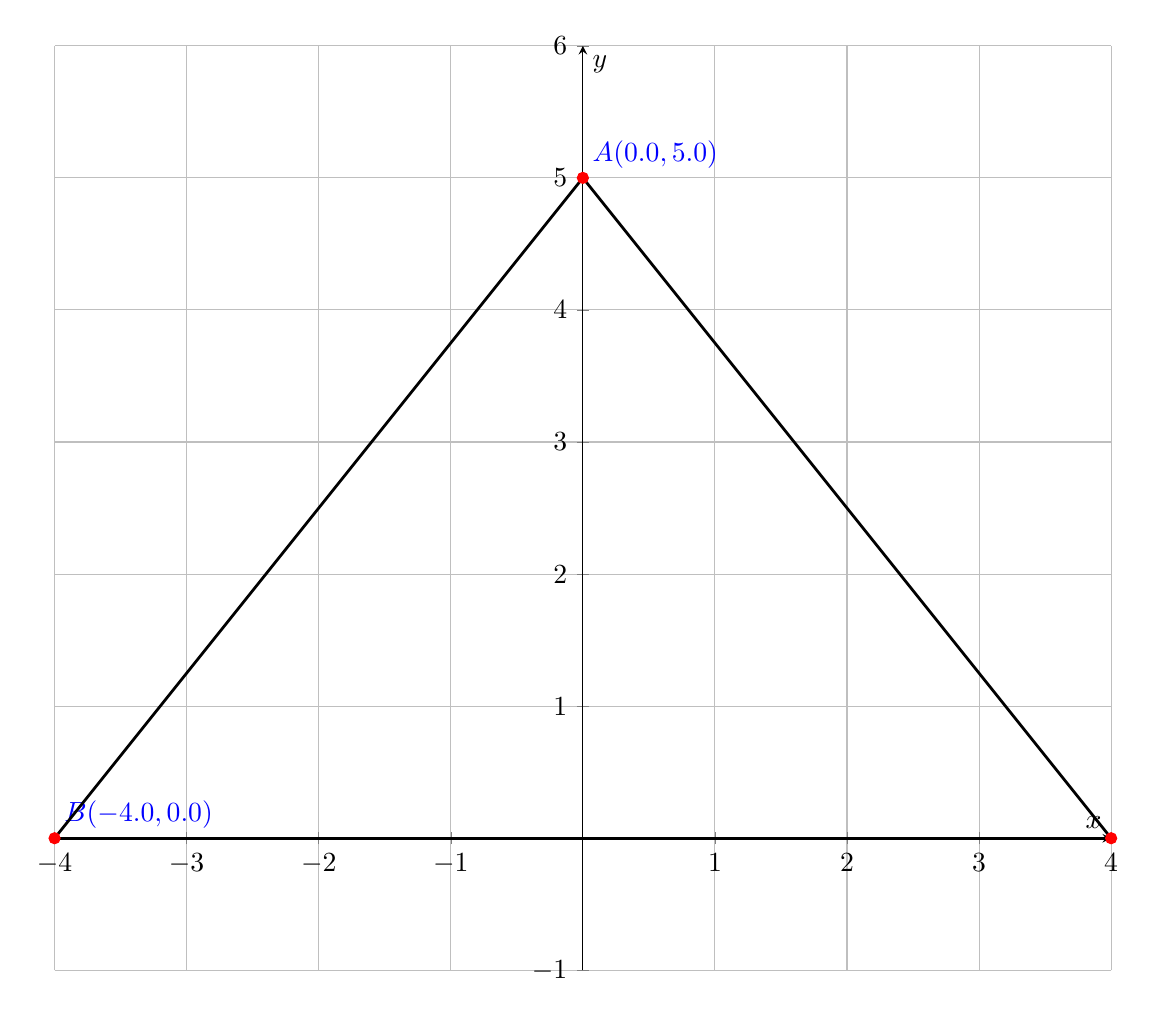
\begin{tikzpicture}

\pgfmathsetmacro{\h}{5.0}

\pgfmathsetmacro{\b}{4.0}
\begin{axis}[
            width=15cm,
            height=15cm,
            axis equal image,
            axis lines=middle,
            grid=major,
            enlargelimits=false,
            clip=true,
            xlabel=$x$,
            ylabel=$y$,
            domain=-6.0:6.0,
            ymin=-1.0,ymax=6.0,
            view={0}{90},
            samples=200
            ]
        

            \addplot[only marks, mark=*, mark size=2pt, color=red] coordinates {({0.0},{5.0})};
            \node[blue, above right] at (axis cs:{0.0},{5.0}) {$A({0.0}, {5.0})$};
        

            \addplot[only marks, mark=*, mark size=2pt, color=red] coordinates {({-4.0},{0.0})};
            \node[blue, above right] at (axis cs:{-4.0},{0.0}) {$B({-4.0}, {0.0})$};
        

            \addplot[only marks, mark=*, mark size=2pt, color=red] coordinates {({4.0},{0.0})};
            \node[blue, above right] at (axis cs:{4.0},{0.0}) {$C({4.0}, {0.0})$};
        
\addplot[line width=1pt, black] coordinates {({-4.0},{0.0}) ({0.0},{5.0})};
\addplot[line width=1pt, black] coordinates {({0.0},{5.0}) ({4.0},{0.0})};
\addplot[line width=1pt, black] coordinates {({-4.0},{0.0}) ({4.0},{0.0})};
\end{axis}
\end{tikzpicture}
\end{center}

\end{document}
